\documentclass[11pt]{article}
\usepackage[utf8]{inputenc}
\usepackage[T1]{fontenc}

% margins
\usepackage[margin=2cm]{geometry}

% graphics path
\usepackage{graphicx}

% use tabu instead of tabular
\usepackage{tabu}
\tabulinesep=1.5mm

% useful math stuff
\usepackage{amsmath, amsfonts, amssymb, amsthm}

% set graphics path
\graphicspath{ {./} }

% define colors
\usepackage{xcolor}
\definecolor{codegreen}{rgb}{0,0.6,0}
\definecolor{codegray}{rgb}{0.5,0.5,0.5}
\definecolor{codepurple}{rgb}{0.58,0,0.82}
\definecolor{backcolour}{rgb}{0.95,0.95,0.92}

% use noto monspace as the monospace font
\usepackage{noto-mono}

% lstlisting and lstinline for code (also sets style for lstlisting env)
\usepackage{listings}
\lstdefinestyle{mystyle}{
    backgroundcolor=\color{backcolour},
    commentstyle=\color{codegreen},
    keywordstyle=\color{magenta},
    numberstyle=\tiny\color{codegray},
    stringstyle=\color{codepurple},
    basicstyle=\ttfamily\footnotesize,
    breakatwhitespace=false,
    breaklines=true,
    captionpos=b,
    keepspaces=true,
    numbers=left,
    numbersep=5pt,
    showspaces=false,
    showstringspaces=false,
    showtabs=false,
    tabsize=2
}
%\lstset{
%    style = mystyle,
%    inputencoding = utf8, % input encoding
%    extendedchars = true, % extended ASCII
%    literate = % support addition characters (https://tex.stackexchange.com/a/574950)
%        {λ}{{$\lambda$}}1
%        {∀}{{$\forall$}}1
%        {Ö}{{\"O}}1
%        {∧}{{$\land$}}1
%        {∨}{{$\lor$}}1
%        {_}{{\_}}1
%        {β}{{$\beta$}}1
%        {γ}{{$\gamma$}}1
%        {∈}{{$\in$}}1
%        {→}{{$\to$}}1
%        {⇒}{{$\implies$}}1
%        {ε}{{$\varepsilon$}}1
%        {≡}{{$\equiv$}}1
%        {ℕ}{{$\mathbb{N}$}}1
%        {×}{{$\times$}}1
%}


\usepackage{tabto}

\newenvironment{tabs}[1]
 {\flushleft\TabPositions{#1}}
 {\endflushleft}

% make toc references clickable (also adds \href and \url) (near last import)
\usepackage{hyperref}
\hypersetup{
    colorlinks=true,
    linkcolor=blue,     % internal link colors
    filecolor=magenta,  % links to local files
    urlcolor=blue,      % links to web addresses
}


% tikz for drawing trees
% Note: may find simplified packages like tikz-qtree and forest useful
\usepackage{tikz}

% add \argmax and \argmin
\DeclareMathOperator*{\argmax}{arg\,max}
\DeclareMathOperator*{\argmin}{arg\,min}

% allow matrices to contain up to 30 columns
\setcounter{MaxMatrixCols}{30}

% disable automatic indent and add horizontal space between two paragraphs
\newlength{\newindent}
\setlength{\newindent}{\parindent}
\setlength{\parindent}{0pt}
\renewcommand{\indent}{\hspace\newindent}
\usepackage{parskip}

% disable toc section numbers
\setcounter{secnumdepth}{0}

% set toc title
\renewcommand*\contentsname{Table of Contents}

\begin{document}
Link to project: \url{https://github.com/koitu/cs348-project}

\section{Description}
%Our proposed application is a comprehensive sports database, potentially focusing on soccer, that will contain detailed information on players, teams, games, and statistics. The aim of the application is to provide easy access to the data stored in the database for sports enthusiasts. The database management system will be designed to be maintained and administered by sports teams or organizers.\\

The proposed application for this project is a comprehensive National Hockey League (NHL) database for game and player statistics from the 2008-2009 season until the current season. The application itself will be a web app focused on getting simple to advanced statistics on players and teams, allowing for an easy user experience when retrieving the data. The aim is to provide a simple way for hockey enthusiasts to look up whatever data they need. The database management system will be designed such that there are administrators who can modify any type of data, team accounts that can modify the data of their team, and users that can simply query the database. \\

The functionalities that will be supported include searching for individual players and their statistics. This includes stats accumulated in an arbitrary time period, specific games where certain stats were met, and so on. Similar queries will be supported for team searches just with team-specific stats, such as wins between time periods, wins against certain opponents, and so on. An account system with certain saved queries and personalized information will also be supported for the users of the application. This allows certain important and potentially expensive queries to be cached to improve the usability of the app.


\section{System Support}
Currently, the application is a web-based app that runs on Windows, MacOS, and Linux currently using local hosts for the frontend and backend sides. This allows for simple launching, testing, and demonstrating of the web app. It would be possible to use a remote server and have the app operate as a more typical website, however, this is an additional step and could realistically only be implemented in later steps, if at all. The programming frameworks chosen are Flask (Python-based web framework) for the backend and React (Javascript-based runtime environment) for the frontend. \\

The database used in this project will be locally hosted. Again this is for ease of use, testing, and demonstration. It would be possible to host the database on a remote server, and this could be implemented in later milestones. The database will use MySQL as the DBMS to query the database, allow different users to log in, and other database features. Python has MySQL packages which makes the implementation of queries simple on the backend. \\ 

\section{Data Gathering}
The current plan for getting both toy and sample data is to use and reformat the data held in this NHL, database https://moneypuck.com/data.htm. This database holds detailed statistics from games played from 2009 to the present day. The database also has detailed player information. This database has some redundant information, and its current schema must be modified to match our current schema. The database also uses .csv files which will need to be converted to an appropriate SQL file. However these are minor changes, and the sheer volume of data is exactly what is needed for this project, and this will be the primary source of data. \\

We will use 3 or 4 players and 3-4 sample teams from the same season for the sample data. This will provide enough information to run the sample queries. \\

The source used also updates its data regularly, so there must be methods in place to update the database to obtain new data. A solution to this problem is to have the DBMS fetch and update the tables from the source. This could be done manually or scripted to automatically update if the data is too old. This approach could help with the final database, however, it will not be implemented for the sample data as there is plenty of data to use already. \\

%he application will be designed to operate on a local machine. The user interface will be implemented using a web interface, which will provide users with an intuitive and user-friendly experience.\\

\section{Database Design}

Assumptions made about the data being modeled:
\begin{enumerate}
    \item Players ids are all unique
    \item Team ids are all unique
    \item Game ids are all unique
    \item Accounts will either be users or admins, not both or neither.
    \item A player in a game is playing on either the home or away team, but not both or neither.
\end{enumerate}

\begin{center}
    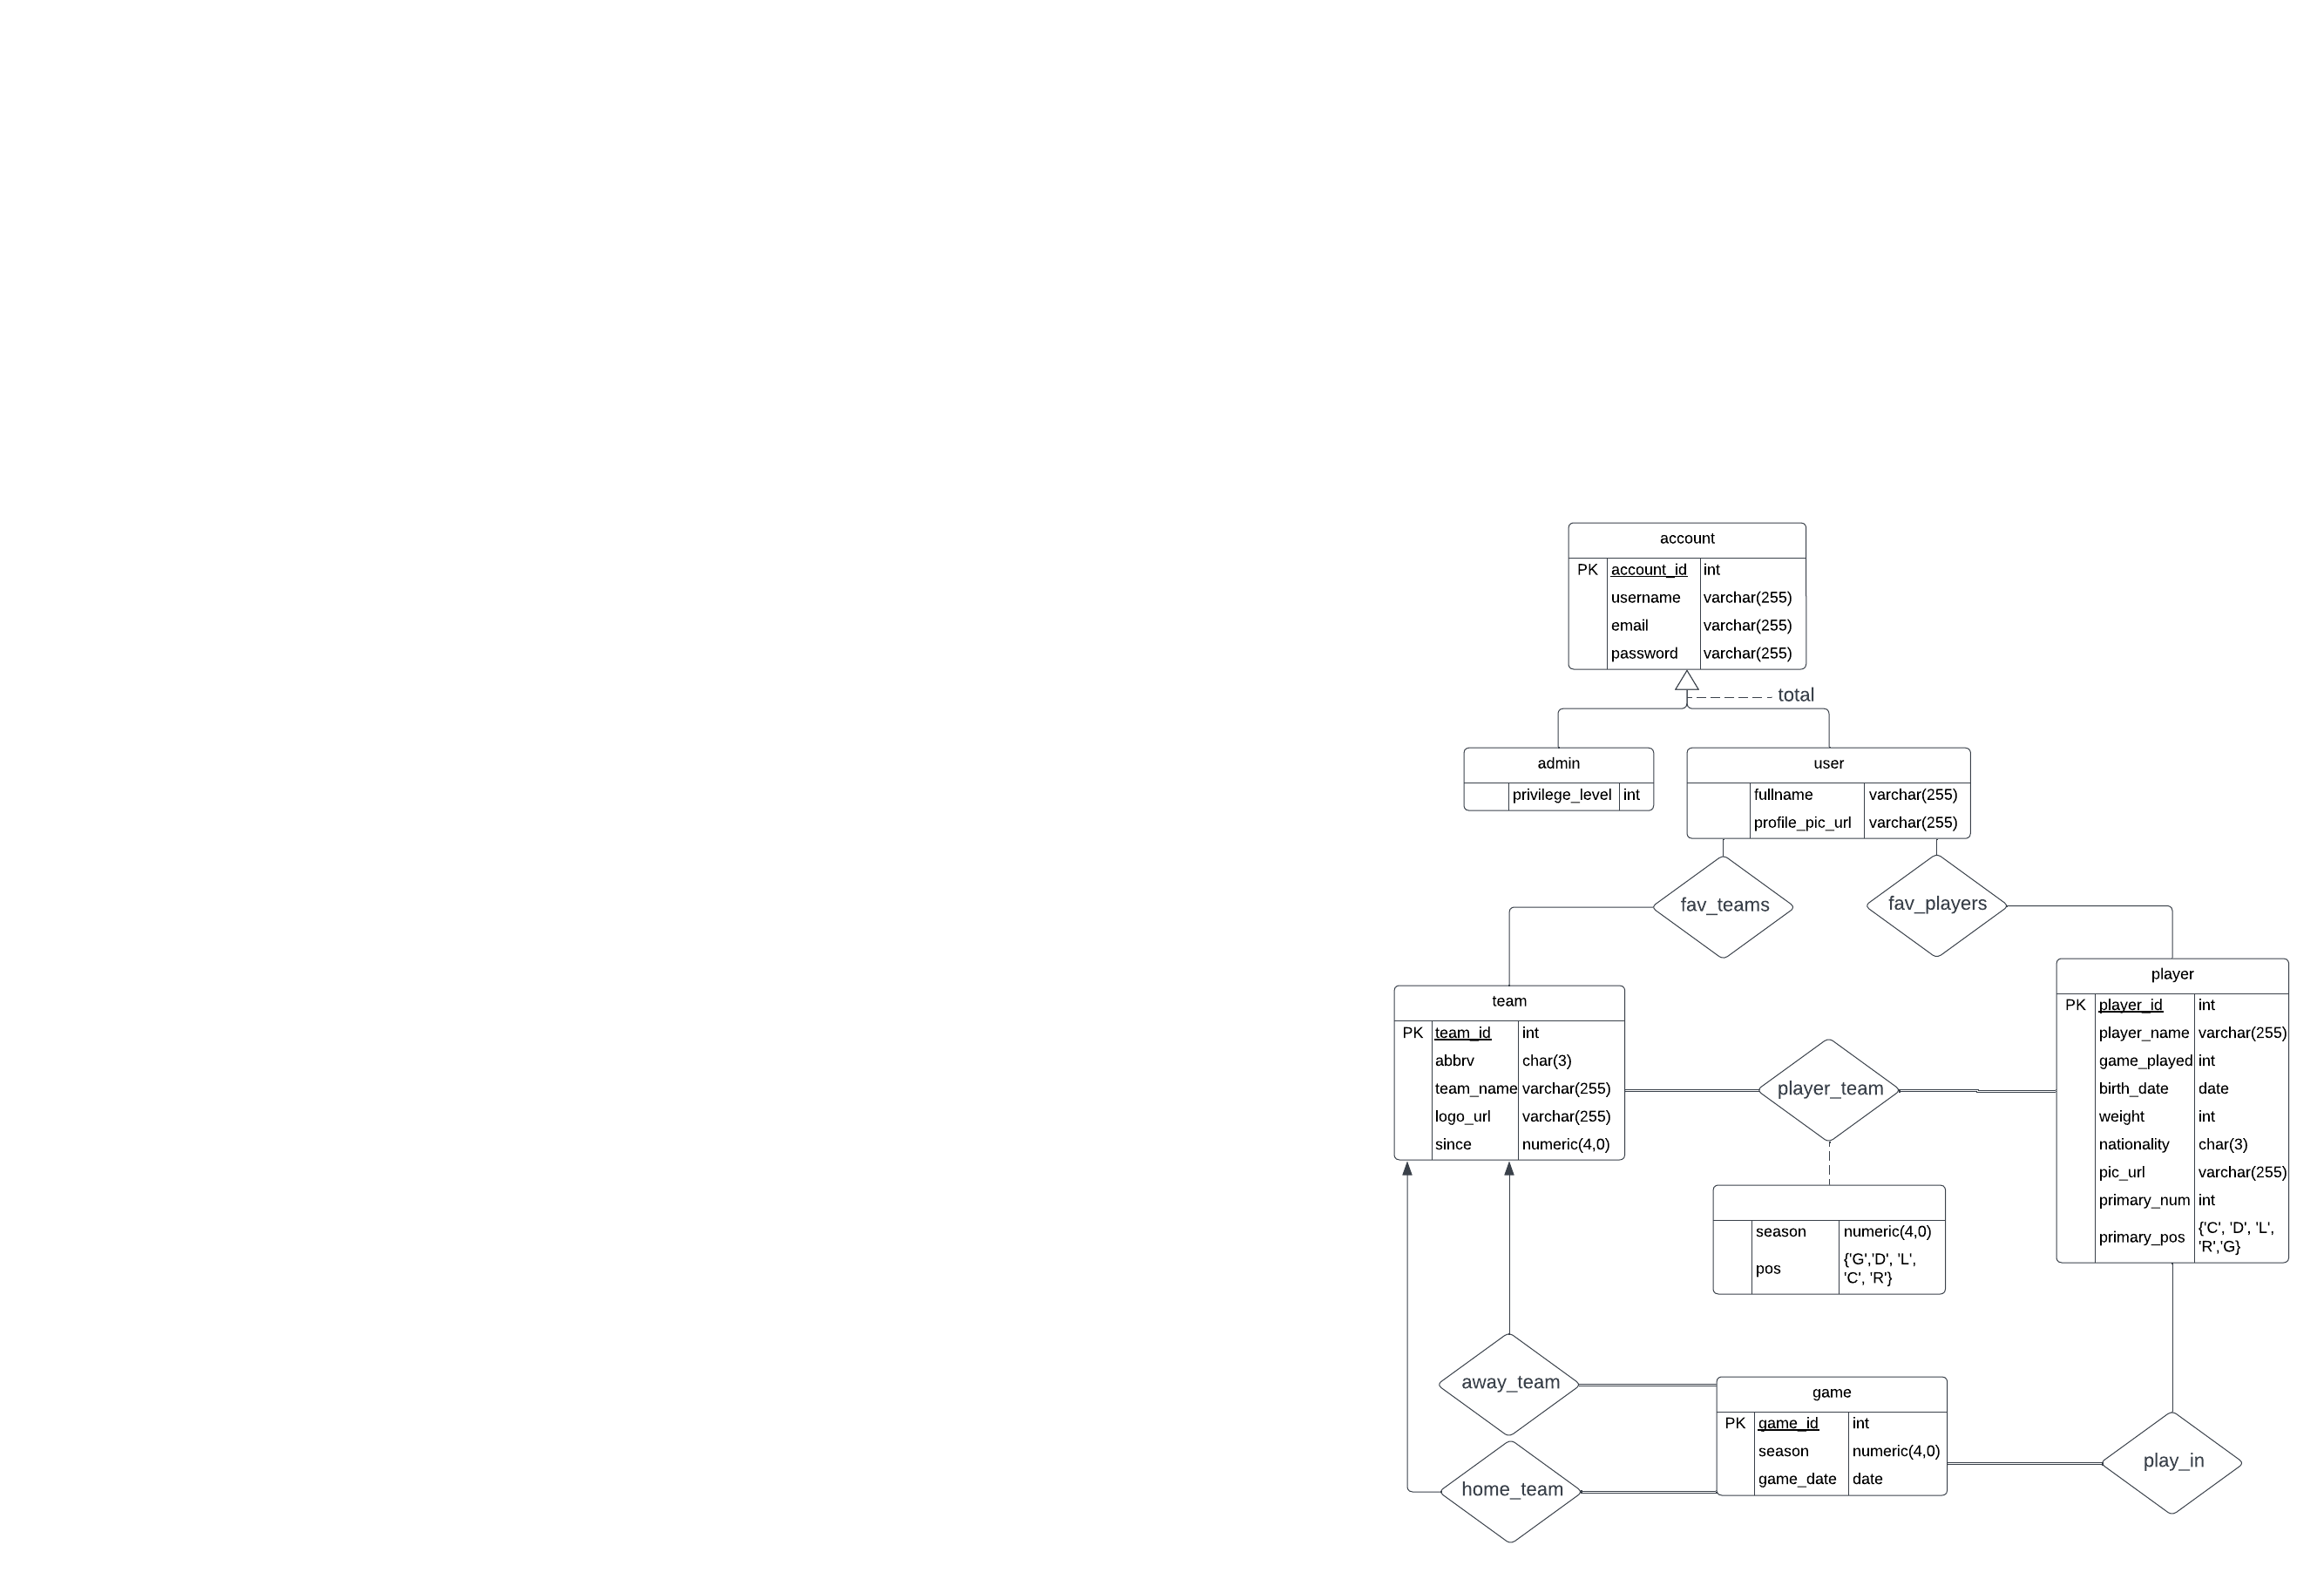
\includegraphics[width=1\textwidth]{ER_Diagram.png}
\end{center}


\vspace{40mm}
\begin{tabs}{1cm,2cm}
Admin(\underline{account\_id}, username, email, password, privilege\_level) \\
\vspace{4mm}
User(\underline{account\_id}, username, email, password, fullname, profile\_pic\_url)\\
\vspace{4mm}
Fav\_Teams(\underline{uid, tid})\\
. \tab \textbf{Foreign Key:} uid references account\_id in User\\
. \tab \textbf{Foreign Key:} tid references team\_id in Team\\
\vspace{4mm}
Fav\_players(\underline{uid, pid})\\
. \tab \textbf{Foreign Key:} uid references account\_id in User\\
. \tab \textbf{Foreign Key:} pid references player\_id in Player\\
\vspace{4mm}
Player(\underline{player\_id}, player\_name, games\_played, birth\_date, weight, nationality, pic\_url, primary\_num, primary\_pos) \\
\vspace{4mm}
Team(\underline{team\_id}, abbrv, team\_name, logo\_url, since) \\
\vspace{4mm}
Player\_team(\underline{pid, tid}, season, pos) \\
. \tab \textbf{Foreign Key:} pid references player\_id in Player \\
. \tab \textbf{Foreign Key:} tid references team\_id in Team \\
\vspace{4mm}
Play\_in(\underline{pid, gid}) \\
. \tab \textbf{Foreign Key:} pid references player\_id in Player \\
. \tab \textbf{Foreign Key:} gid references game\_id in Game \\
\vspace{4mm}
Game(\underline{game\_id}, season, game\_date, homeid, awayid) \\
. \tab \textbf{Foreign Key:} homeid references team\_id in Team \\
. \tab \textbf{Foreign Key:} awayid references team\_id in Team \\
\vspace{4mm}
\end{tabs}


\section{Feature Descriptions}


\begin{enumerate}

\item Searching for players is one feature of the application. In the search bar you can type in a string and any players whose names have a matching substring will appear in the results. The results will be links to the player's page which will then have detailed stats about them. This allows the application to work almost as a search engine. In the future, an algorithm on the backend can detect typos and attempt to return the closest matches. A simple example is case-insensitive searching. Extra clauses can be added to the where section of the query for filtering. \\

The template query goes as follows. Note that currently, the sample query returns all the attributes associated with the player. This can be modified to only return the necessary attributes, or fancy features can make use of these attributes. Also, note that seasons will be an optional join that will only join on the specified seasons in the future.

\begin{verbatim}
    select *
    from Player
    where player_name like '%<searched string>%' <optional filters here>
\end{verbatim}

As a sample query:
\begin{verbatim}
    select *
    from Player
    where player_name like '%Alex%' and age >= 30
\end{verbatim}

A useful feature of this is that with an empty substring, all players will be returned. This allows for finding players based on these optional filters. \\


\item Searching for teams is another feature of the application similar to searching for players. The search result will return teams instead. Filters can be used to narrow down teams, however, the filters will now be different. Teams can be viewed as one team, or if a year filter is selected the teams from just those seasons will appear. \\

The template query goes as follows, again the same nuances apply to the returned attributes.
\begin{verbatim}
    select *
    from Team
    where team_name like '%<searched string>%' <optional filters here>
\end{verbatim}

As a sample query:
\begin{verbatim}
    select *
    from Team
    where team_name like '%New%' and since <= 2000
\end{verbatim}

\item A player's team will be retrieved and shown on the player's personal page.\\ 

A template query goes as follows:
\begin{verbatim}
    with T as (select *
               from Player
               where player_id = <current_player>)
    select team_name
    from T natural join player_team natural join Team
\end{verbatim}

As a sample query:
\begin{verbatim}
    with T as (select *
               from Player
               where player_id = 123)
    select team_name
    from T natural join player_team natural join Team
\end{verbatim}

\item On a player page, there will be a section for recent games played. These games will be retrieved from the database. Initially only the 5 most recent games will be shown, subject to the constraints given by the filter from the search. This can be changed later on the add an option to show more games. \\

The template query goes as follows:

\begin{verbatim}
    with T as (select *
               from Player
               where player_id = <current_player>)
    select *
    from T natural join play_in natural join Game
    order by game_date desc
    limit 5
\end{verbatim}

As a sample query:

\begin{verbatim}
    with T as (select *
               from Player
               where player_id = 123)
    select *
    from T natural join play_in natural join Game
    order by game_date desc
    limit 5
\end{verbatim}

\item The next feature is for users to add favorites to their favorites player page. This will allow users to quickly access the players they want most. This feature can also be quickly changed to allow for favorite teams pages to be saved. \\
The template query goes as follows:
\begin{verbatim}
    insert into fav_players
    values (<current_user_id>, <player_id>)
\end{verbatim}

As a sample query:
\begin{verbatim}
    insert into fav_players
    values (987, 123)
\end{verbatim}
\end{enumerate}

\section{Members}
\begin{itemize}
    \item Andrew Wang (20882272). Responsible for the front-end and back-end implementations and implementing queries.
    \item Shayan Mohammadi Kubijari (20967990). Responsible for schema design, query implementations, and converting the database to SQL, along with modifying the database to fit the schema.
    \item Arvin Asgharian Rezaee (20972431). Responsible for the front-end and back-end implementations, setting up the scripts to launch the project and query implementation.
    \item Victor Astinov (20851407). Responsible for the template queries, documentation, and sourcing of the database.
    \item Shang Jin (21051963). Responsible for the schema design, ER diagrams, and relational data model.
\end{itemize}

All team members did their part as expected. The progress made for all team members is the expected progress for milestone 1.


\end{document}
